\documentclass[12pt]{article}
% Packages
\usepackage[utf8]{inputenc}
\usepackage[T1]{fontenc}
\usepackage[margin=1in]{geometry}
\usepackage[UKenglish]{babel}% http://ctan.org/pkg/babel
\usepackage[UKenglish]{isodate}% http://ctan.org/pkg/isodate
\usepackage{amsmath, amsthm, amsfonts, amssymb}
\usepackage{mathrsfs}           % \mathscr font.
\usepackage{setspace}
\usepackage[colorlinks=true,
    linkcolor=red,
    citecolor=red,
    urlcolor=red,
    breaklinks]{hyperref}
\usepackage{graphicx}
\usepackage{booktabs}
\usepackage{subcaption}
\usepackage{xcolor}
% \usepackage[style = authoryear, autocite=inline, doi=false,isbn=false,url=false]{biblatex}
\usepackage{natbib}
% \usepackage{libertine}

% \usepackage[sf]{titlesec} % make section headings \sffamily

% Header styling
% make headers \sffamily
% \newpagestyle{main}[\sffamily]{
%     \sethead{\thepage}{}{\sectiontitle}
%     }
% \pagestyle{main}
\usepackage{titling}
% make titling elements \sffamily
% \pretitle{\begin{center}\sf \LARGE}
% \preauthor{\begin{center}
%             \large \lineskip 0.5em%
%             \begin{tabular}[t]{c}}
% \predate{\begin{center}\large}
\usepackage{abstract}
% make abstract title \sffamily
% \titleformat{\section}[block]{\Large \bf \sffamily}{\thesection}{1em}{}
\usepackage{caption}
\captionsetup{labelfont = bf}

\usepackage{longtable}
\usepackage{dcolumn}
\usepackage[toc,page,header]{appendix}
\usepackage{minitoc}
\usepackage{booktabs}
\usepackage{longtable}
\usepackage{array}
\usepackage{multirow}
\usepackage{wrapfig}
\usepackage{float}
\usepackage{colortbl}
\usepackage{pdflscape}
\usepackage{tabu}
\usepackage{threeparttable}
\usepackage{flafter}
\usepackage{threeparttablex}
\usepackage[normalem]{ulem}
\usepackage{makecell}
\usepackage{xcolor}
\usepackage{color, colortbl}
\definecolor{lgrey}{gray}{0.9}
\usepackage{siunitx}
\sisetup{
    detect-all,
    round-integer-to-decimal = true,
    group-digits             = true,
    group-minimum-digits     = 4,
    group-separator          = {\,},
    table-align-text-pre     = false,
    table-align-text-post    = false,
    input-signs              = + -,
    input-symbols            = {*} {**} {***},
    input-open-uncertainty   = ,
    input-close-uncertainty  = ,
    retain-explicit-plus,
    parse-numbers = false
}
\newcolumntype{d}[1]{D..{#1}}


\usepackage{etoolbox}

\makeatletter

% Patch case where name and year are separated by aysep
% \patchcmd{\NAT@citex}
%   {\@citea\NAT@hyper@{%
%      \NAT@nmfmt{\NAT@nm}%
%      \hyper@natlinkbreak{\NAT@aysep\NAT@spacechar}{\@citeb\@extra@b@citeb}%
%      \NAT@date}}
%   {\@citea\NAT@nmfmt{\NAT@nm}%
%    \NAT@aysep\NAT@spacechar\NAT@hyper@{\NAT@date}}{}{}

% % Patch case where name and year are separated by opening bracket
% \patchcmd{\NAT@citex}
%   {\@citea\NAT@hyper@{%
%      \NAT@nmfmt{\NAT@nm}%
%      \hyper@natlinkbreak{\NAT@spacechar\NAT@@open\if*#1*\else#1\NAT@spacechar\fi}%
%        {\@citeb\@extra@b@citeb}%
%      \NAT@date}}
%   {\@citea\NAT@nmfmt{\NAT@nm}%
%    \NAT@spacechar\NAT@@open\if*#1*\else#1\NAT@spacechar\fi\NAT@hyper@{\NAT@date}}
%   {}{}

\makeatother

% Define symbols and maths shortcuts
\DeclareRobustCommand{\bbone}{\text{\usefont{U}{bbold}{m}{n}1}}
\DeclareMathOperator{\EX}{\mathbb{E}} % expected value
\DeclareMathOperator{\V}{\mathbb{V}}
\DeclareMathOperator{\Prob}{\mathbb{P}}
\newcommand*{\trans}{^{\mathsf{T}}} %matrix transpose



\usepackage{booktabs}
\usepackage{longtable}
\usepackage{array}
\usepackage{multirow}
\usepackage{wrapfig}
\usepackage{float}
\usepackage{colortbl}
\usepackage{pdflscape}
\usepackage{tabu}
\usepackage{threeparttable}
\usepackage{threeparttablex}
\usepackage[normalem]{ulem}
\usepackage{makecell}
\usepackage[toc,page,header]{appendix}
\usepackage{xcolor}
\usepackage{siunitx}
\usepackage{chngcntr}
\usepackage{minitoc}
\usepackage{caption}
\usepackage{setspace}
\usepackage[hang]{footmisc}
\captionsetup{font = small}

% Make the "Part I" text invisible
\renewcommand \thepart{}
\renewcommand \partname{}

\setlength\labelsep{0pt}

\title{The Gender Gap in Political Careers \\ Under Proportional Representation}
\date{April 2023}
\date{}
\author{Tobias Nowacki\thanks{Senior Data Scientist, Deliveroo. I thank Kirk Bansak, Chris Berry, Gary Cox, Andy Eggers, Jon Fiva, Olle Folke, Ignacio Lago, Justin Grimmer, Andy Hall, Apoorva Lal, Sandy Handan-Nader, Jens Hainmueller, Jonathan Rodden, Brett Parker, Tine Paulsen, Soledad Prillaman, Johanna Rickne, Dan Smith, Dan Thompson, and participants in the Democracy and Polarization Lab and at the APSA 2021 panel for helpful comments.}}

% \addbibresource{Spain_Careers.bib}


% Begin Document
\begin{document}

%
% FRONT PAGE -----------------------------------------------------------------
%

\renewcommand \thepart{}
\renewcommand \partname{}

\maketitle
\thispagestyle{empty}

\begin{center}
    {Conditionally Accepted at the Journal of Politics}
\end{center}

\singlespacing
\begin{abstract}
    Does proportional representation feature gender gaps in incumbency advantages?  I argue that closed-list PR (compared to open-list PR) can help to attenuate the gender difference by reducing voters' influence over individual candidates' electoral outcomes. Using difference-in-discontinuity designs, I contrast gender-specific incumbency effects in municipal elections across Norway (open-list) and Spain (closed-list). In Norway, women experience an incumbency advantage in winning future elections that is up to 60\% smaller than men's; in Spain, female candidates enjoy incumbency effects equal to or greater than men's. Additional results suggest that these findings are unlikely to be due to unobserved country characteristics or differential selection. Although more suggestive, further evidence is consistent with voter bias entering through preference votes for individual candidates -- especially in right-wing parties -- as a key mechanism for the gender gap in open-list PR. All told, this paper highlights the importance of electoral rules in ensuring gender equity in political representation by addressing leaky pipelines in office.
\end{abstract}

Keywords: incumbency advantage; gender gap; local elections; proportional representation; electoral systems

\doparttoc % Tell to minitoc to generate a toc for the parts
\faketableofcontents % Run a fake tableofcontents command for the partocs

\part{} % Start the document part
% \parttoc % Insert the document TOC


\clearpage
\pagenumbering{arabic}
\doublespacing

%
% MAIN BODY -----------------------------------------------------------------
%

% --------------------
% SECTION 1 - INTRO
% --------------------


Women are underrepresented in politics, which is concerning for intrinsic normative reasons, as well as for its consequences for policy outcomes after the election is realised \citep{mansbridge1999, mansbridge2003,chattopadhyay2004,dahlerup2013}. A rich literature explains the empirical fact that countries using proportional representation (PR) are more likely to feature higher proportions of women elected to the legislature -- and thus less `sticky' floors \citep[][]{norris1985,matland1996,matland1998,thames2010,roberts2013,casas-arce2015,thames2016,golder2017a,verge2019a,lucardi2020,profeta2022}. Yet, simply counting the number of women elected to the legislature is insufficient for achieving gender equity in politics: their career trajectory, time in office, and political experience, as well as their efficiency as policymakers representing women's preferences all matter for this objective \citep{smrek2020}. If female officeholders suffer from a `leaky pipeline' \citep{cipullo2021} in their careers -- that is, once elected, they are still less likely to win re-election and promotion to higher offices -- concerns about unequal representation persist.

Do PR systems struggle with a gender gap in political career trajectories? More specifically, is there a gender gap in the effect of incumbency on re-election and future career outcomes?

In this paper, I study how different forms of PR (open versus closed-list) shape the gender gap in the effect of winning office on future election outcomes -- typically the next step in the career trajectory after winning office. I argue that elections using closed-list PR -- compared to those with open-list PR -- are more likely to plug the 'leaky pipeline' by limiting voters' influence over individual candidates' ranking, which may otherwise disadvantage women disproportionately due to voter or systemic bias. In closed-list PR, incumbency advantages arise from party elites' decisions to elevate candidates throughout list ranks. Though party elites may have initial negative biases against women, they have little reason to treat bare winners (compared to bare losers) differentially by gender \citep{luhiste2015,hazan2006a}.\footnote{If anything, their initial bias towards women should diminish upon observing them perform in office \citep{kjaer2019}} By contrast, in open-list systems, the effect of being elected on future election outcomes may be differentially greater for men due to a larger increase in personal votes for barely elected male candidates. This gap will be especially pronounced where voters are biased against women, or systemic disadvantages (e.g., smaller name recognition bonuses for women as an effect of incumbency) exist. Overall, this framework implies that women may face diminished incumbency effects in open-list PR systems, while we can expect an equal or even greater incumbency advantage for women in closed-list PR systems. This argument regarding \emph{incumbency advantages} stands in contrast to recent work investigating whether different electoral systems or kinds of PR can improve overall levels of female representation \citep{stegmaier2014women,golder2017a}.

Empirical results from difference-in-discontinuity designs in municipal elections -- typically the first rung in the political career ladder \citep{cirone2020} -- in Norway and Spain are consistent with the theoretical argument. The results support the claim that voter or systemic bias against female candidates can hamper their incumbency advantage in more candidate-centric variants of PR.

In Norway's open-list elections, barely elected women enjoy a significantly smaller incumbency advantage compared to their male colleagues.\footnote{This result is further supported by aggregate descriptive statistics: the general incumbent re-election rate in Norway's local elections stands at 46.6\% for men, while for women, it is 38.2\%.} Whereas men who barely won (compared to men who barely lost) have an approximately 10 percentage point higher probability of winning in the next election, the effect decreases to about 4 percentage points for women who barely won (compared to women who barely lost) -- a 60\% decline vis-a-vis men.\footnote{\label{fn:norway_system}

Voters award preference votes to candidates, which determines their list ranking within the set of candidates fielded by the party. Voter preferences have a meaningful impact on deciding what candidates get elected: \citet{bergh2010} estimate about 25\% of candidates won office because voters' preference votes, rather than list ranking.
While more complex classifications of PR systems may describe Norway's system as `flexible-list' or `semi-open list', I follow the existing literature that recognizes Norway's municipal elections as 'open-list' \citep{fiva2018a, fiva2018b}.} Women in Spain's closed-list elections, by contrast, likely enjoy a differentially greater incumbency advantage than their male colleagues. Importantly, I find no evidence of large gender gaps in career \emph{persistence} in either setting: the effect of winning on the probability of running again is likely similar for men and women in either country.

I supplement the difference-in-discontinuity design with additional evidence to guard against concerns about case selection and differential selection into the threshold sample. While the difference-in-discontinuity design causally identifies the incumbency advantage within each gender, male and female candidate threshold samples may differ in individual-level (age, experience) as well as election-level and geographic attributes. I find that the magnitude of the gender gap in open-list persists when restricting the comparison to female candidates and the most similar male candidate with respect to age, experience and election year in the same party and county.

Second, if the magnitude of differential selection varies across cases, my contrast between open-list and closed-list PR may be an artefact of case selection. To address this concern, I leverage both within- and cross-country variance in electoral rules using data from Norway and Poland to show that the contrast between open- and closed-list PR, rather than idiosyncratic country effects, can explain the gender gap in incumbency advantages.

Finally, I provide suggestive evidence for the theorized mechanism behind the negative gender gap in Norway -- voters awarding a smaller increase in preference votes to barely elected women as a result of attaining incumbency.
Specifically, although women are unlikely to face a differential penalty imposed by their \emph{party} for being elected \citep{kjaer2019}, the effect of winning in right-wing parties results in a far smaller increase, or potentially even decrease, in personal preference votes cast by voters for women when compared to men. Notably, no such discrepancy exists among candidates in left-wing parties, whose voters are more positively predisposed towards women in local politics. Voters' influence over list ranking -- the key difference between open and closed-list PR -- thus likely contributes to the stark difference in incumbency advantage gender gaps across PR systems. Altogether, although suggestive, the evidence in this paper emphasizes the role that voter or systemic biases can have in influencing incumbency advantages where the electoral system is more candidate-centric.

This paper connects and contributes to a number of existing literatures. It offers a new explanation for how electoral rules can affect gender equity in politics \citep{krook2014,obrien2016,krook2018,luhiste2015}.
Although existing work suggests that voter biases that affect women's \emph{unconditional} probability of being elected in the first place may be context- and election-specific \citep{folke2016a, anzia2019, beaman2009,broockman2020,eymmoud2017}, this paper is the first that documents and highlights the contrast in incumbency gender gaps across open- and closed-list PR using difference-in-discontinuity designs. In doing so, it also, for the first time, documents a greater incumbency advantage for women than for men under closed-list PR. It also contributes the use of an RD-style design on intermediate outcomes to provide suggestive evidence for the role of voter or systemic bias in open-list PR. More generally, it adds to a growing literature of works that study how candidates' gender affects incumbency advantage mechanisms under PR \citep{schwindt-bayer2005,jankowski2019,smrek2020}, and whether voters reward incumbency differentially by gender.

Beyond making the important distinction between open- and closed-list PR, the paper also offers a benchmark to evaluate the incumbency gender gap in PR systems against plurality \citep{wasserman2020, cipullo2021, brown2019}. Finally, the paper speaks to the broader literature on political careers \citep{cirone2020,kerevel2019,folke2014} and offers an important theoretical distinction between the mechanisms driving incumbency advantages in open and closed-list PR systems more generally.



% ----------------------------
% SECTION 2 -- LIT AND THEORY
% ----------------------------

\section{Electoral Systems and the Gender Gap in Political Careers}


\subsection{PR Boosts Number of Women Running (and Winning)}

Proportional representation (PR) can boost the number of female candidates running (and potentially winning) for a number of reasons: Where party elites have control over nominations, they may follow gender-agnostic seniority norms \citep{fiva2018a,cirone2020}; incumbency advantages are less severe than in plurality, thus allowing ascending women to replace men more easily \citep{fiva2018b,meserve2020}; in multi-member districts, nominating elites no longer have to cater to the `lowest common denominator' and can instead attempt a more equitable distribution of viable spots within a district \citep{matland1998}. Additional work also finds that open-list systems are particularly suitable for enhancing the share of women elected \citep{stegmaier2014women,golder2017a}, although the design limitations of these works cannot establish a clear causal effect from electoral system to female representation. Finally, PR systems can allow for a more fragmented party system in which left-leaning parties with a strong emphasis on gender equity push forward with nominating more women into viable spots, and other parties are forced to follow \citep{matland1996}.

Although increasing women's numerical representation on the ballot and in office is essential for ensuring equity in downstream policy outcomes - such as fiscal policy \citep{bagues2020} -- it is not sufficient on its own. While existing work points towards PR attenuating the problem of a ``sticky floor'' for women, it remains an open question whether it can also close the ``leaky pipeline'' along women's career trajectories \citep{cipullo2021}. This question is distinct from whether voters or parties treat female candidates differently unconditionally: once the conditional set of successful candidates is elected, male and female candidates may still interact differently with a given electoral system's incumbency advantage and career promotion mechanisms. This point is especially important at a time when the overall share of women elected to legislatures has risen across Europe's democracies (see Figure \ref{fig:csts_plot}), but far less is known about the other dimensions of gender equity in politics mentioned above. While scholars have begun to document this type of gender gap in plurality \citep{wasserman2020,cipullo2021}, little work on PR systems has emerged yet.

\begin{figure}[!htb]
    \centering
    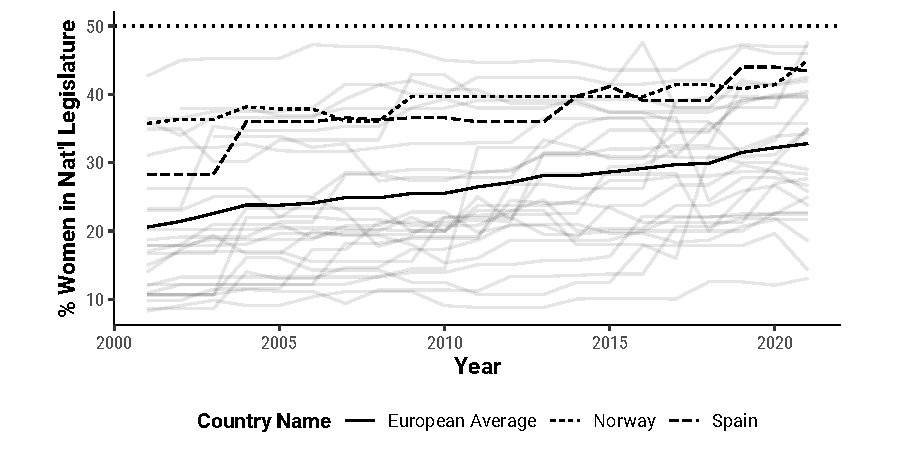
\includegraphics[width = 0.75\textwidth]{../output/figures/csts_plot.pdf}
    \caption{Share of female legislators in national legislatures (lower houses) across European democracies (World Bank, 2023).}
    \label{fig:csts_plot}
\end{figure}

Evaluating the gender gap in political careers under PR is thus important for improving representation and democratic legitimacy. If women, once elected, have shorter tenures in office or miss out on promotion to senior office, their representation might still carry less weight, as they wield less power and experience in legislative processes. Moreover, if women suffer from diminished effects of being elected on future career progression, this might also contribute to a greater gender gap in representation at higher levels of political office.

One key aspect that may drive the gender gap in political careers is whether there is a difference in the effect of being elected on running again and winning again as the most proximate candidate-levels outcomes of winning office. Any gender differential in the effect of being re-elected will have knock-on effects on future downstream career outcomes (such as running for or winning election to the national legislature). Studying this first outcome therefore sheds light on where the `leaky pipeline' begins, and is, so far, understudied for the domain of PR \citep{smrek2020}.

\subsection{When Does PR Create Similar Incumbency Advantages for Men and Women?}

How, if at all, should we expect incumbency advantages under PR to differ by candidates' gender? More candidate-centred (i.e., open-list) systems, in which voters can determine the ranking of individual candidates, may render women more vulnerable to voter and systemic biases, and lead to a smaller incumbency advantage compared to men.

Table \ref{tab:inc_mechanisms} summarizes the argument. The primary incumbency advantage mechanism in closed-list systems -- rank increases due to seniority -- is unlikely to produce a gender gap, even if party elites are unconditionally biased against women. By contrast, a key mechanism in open-list PR systems -- an increase in personal votes due to name recognition -- may be reduced for women and produce a smaller incumbency advantage for female candidates if voters are biased or update less on female incumbents due to systemic bias. Altogether, closed- and open-list PR systems have different mechanisms through which the incumbency advantage operates. This, in turn, affects the gender gap in incumbency advantages -- irrespective of any unconditional differences in how likely men or women are to win office. Below, I elaborate on the incumbency mechanisms and their vulnerability towards gender biases in each setting.

\begin{table}[thbp]
    \centering\begin{tabular}{lcc}
        \toprule
         & \textbf{Closed-list} & \textbf{Open-list} \\
        \cmidrule(lr){1-3}
        Incumbency Effect Mechanisms & & \\
        \, \emph{Party-driven} &  Seniority  & Seniority \\
        & Resource Advantage & Resource Advantage \\
        & (rank advance) & (pre-vote rank advance) \\[2mm]
        \, \emph{Voter-driven}  &                          & Name Recognition  \\
                  & & (pref vote increase) \\[2mm]
       Gender Gap Mechanisms & Social Learning (\textbf{+}) & Social Learning (\textbf{+}) \\
                   & & Voter Bias (\textbf{-}) \\
                   & & Systemic Bias (\textbf{-}) \\
    \bottomrule
    \end{tabular}
    \caption{Main Incumbency Advantage Mechanisms under Proportional Representation}
    \label{tab:inc_mechanisms}
\end{table}

\paragraph*{Closed-list PR.} In closed-list PR, the rank order of list positions decides individuals' electoral fortunes: higher list ranks translate into greater electoral security. Mechanically -- as long as voters' decision what party to vote for does not depend on the position of individual candidates -- any incumbency advantage for barely elected politicians must come from an improved list rank.\footnote{The larger the district magnitude, the easier this assumption becomes to satisfy. With dozens of candidates on a party list, voters are unlikely to switch their ballot to another party because of a single candidate that they dislike.} Put differently, candidates who are just barely elected move up to a safer list position with a higher chance of winning office in the next election. This mechanism is often institutionalized as a seniority norm in closed-list PR systems \citep[cf.][]{cirone2020}. Alternatively, even where no strong official seniority norm exists, incumbents (compared to non-incumbents) may be able to marshal significantly greater resources and stronger networks at their disposal in order to occupy any better ranked list positions when vacancies open up \citep{trounstine2010modern,nunez2018clientelistic}.

Note that party elites may treat male and female candidates quite differently in an unconditional sense: across the whole set of available list positions, they may, on average, rank women in lower positions; they may also assign female candidates to more (or less) competitive districts. There are two primary explanations for this phenomenon: one is that party elites are biased against female candidates themselves (which is discussed below); the other is that they engage in strategic ranking behavior in order to maximize the party's vote share. In practice, however, there is limited evidence that voters -- who cast votes for whole party lists, not individual candidates -- are highly sensitive to the gender composition of the party list \citep{bagues2020a}, especially in elections with high district magnitude.

However, when comparing incumbency advantages among barely elected winners -- that is, thinking about the additional effect \emph{conditional} on winning office -- we need to consider whether party elites' behavior shows any meaningful gender difference in response to getting elected. The question here is no longer whether women experience greater obstacles towards being elected overall, but whether, once they are elected (and in comparison to men in a similar position), they experience similar rank improvements and hence incumbency advantages of a similar magnitude as male candidates.

More specifically, consider two distinct scenarios regarding party elite bias, with different implications for the incumbency gender gap under closed-list PR. First, assume that party elites treat male and female candidates equally across the whole list; hence, both male and female barely elected winners are of the same quality. Quality can, for example, mean greater effectiveness as a policymaker, responsiveness to voters \citep{anzia2011}, or greater success in securing funding for the municipality. Why should the party leadership advance male winners faster towards safer list positions than female winners? One answer could be that parties decide candidate placement strategically in order attract voters who are biased towards or prefer male candidates. If such voters and punish lists with too many women at the top, parties may want to boost male incumbents further and award them more advantageous positions. However, as mentioned before, there is limited evidence party lists that increase the share of women on the list are being punished at the ballot box \citep{bagues2020a}.


Second, party leadership may still exhibit unconditional negative biases towards women -- for example, in the form of lower initial placements or a penalty to their perceived quality \citep{luhiste2015,murray2012,krook2014}. One corollary of this assumption is that female candidates in the sample of barely elected or barely losing candidates will likely be, on average, of higher quality than men in comparable positions \citep{ashworth2021,besley2017}.\footnote{This follows from women having to overcome the bias term in the first place in order to advance to the threshold position, similar to \citet{ashworth2021}.}

If a female candidate who overcomes the initial bias term (e.g. with high quality on the aforementioned dimensions such as lobbying more effectively on behalf of the municipality) and proceeds through the list ranks towards the set of barely elected candidates, it is hard to imagine why parties would further increase their negative bias of women as a result of being elected. Another reason why parties ought to be consistent in their treatment of barely elected candidates is strategic incentives: if the party were to deny women an incumbency advantage (of a similar magnitude as men's), they would be less likely to run and compete in the first place. Put differently, it would be counterproductive to recruit female candidates in the first place, put them in competitive list positions, only to deny them further advancement.

If anything, parties should reduce their negative stereotypes upon observing a female candidate in office perform well: their perception should move closer to the candidate's true ability. If this is the case, and the elites' initial perception was biased downward, women should actually experience a \emph{greater} incumbency advantage than men. Alternatively, female candidates who have overcome initial hurdles and succeeded into the set of list ranks around the election threshold may have greater access to resources and political connections than men of similar list rank -- which female winners may be able to turn into a differentially greater incumbency advantage. An important caveat to this argument is that women may suffer from lower persistence in political careers even after winning elections due to asymmetric outside factors (e.g., higher divorce rates, see \citet{folke2020}), or more general differences in persistence or motivation to run for office \citep{lawless2005, wasserman2020,ashworth2021}).

\paragraph*{Open-list PR.} In open-list (and more candidate-centred) PR systems, part of the incumbency advantage comes from voters awarding elected candidates a boost in preference votes, therefore making it more likely that they will be re-elected \citep{dahlgaard2016, dettman2017, jankowski2021}.\footnote{\citet{fiva2018a}, also studying Norwegian local elections, find the overall effect of incumbency on personal vote shares to be small and statistically indistinguishable from zero. This is likely the result of a particular operationalisation of personal vote share. I discuss this issue further in Appendix \ref{app:norway_pv_estimation} and show that my results -- demonstrating that there is a meaningful effect for male candidates -- hold up across different operationalisations.} In lower-level, low-information elections, such as municipal elections, voters rarely observe the quality of candidates precisely. Instead, they might follow established heuristics in the form of incumbency status, (pre-vote) list rank, and name recognition \citep{dettman2017}. Voters typically only have a limited number of preference votes (e.g. in Norway, one-quarter of the council size) that they can allocate across the party list.\footnote{If parties can still decide the order in which candidates appear on the ballot, they may still be able to affect candidates' success, which is strongly correlated with the initial list position (Appendix \ref{app:pv_by_rank}). In that sense, parties in open-list determine which candidates enter the set of \emph{viable} candidates, but do not have fully discrete power to decide who gets elected.}

In this context, women may experience a diminished incumbency advantage if a subset of voters awards their preference votes to incumbent men, but not women. Consider a pool of voters in which some voters allocate preference votes based on candidates' true quality (perhaps with a noisy, but unbiased signal), while others use name recognition and incumbency as a heuristic; a subset of these heuristic voters only awards preference votes to male incumbents.

Women may still be able to win initial election, carried forward by unbiased voters. However, barely elected men will experience a greater increase in preference votes than barely elected women thanks to male-favoring heuristic voters. (Appendix \ref{app:theorysim} illustrates this argument further with a toy model simulation). With a smaller increase in preference votes, women will also observe a smaller increase in their probability of winning again as an effect of barely winning.\footnote{As in the closed-list case, my theoretical argument does not make a claim about an unconditional difference in candidate type between male and female candidates. If women suffer from a `sticky floor', the entire threshold sample of female candidates may be of higher quality compared to the respective male one. Yet, any alternative explanation focussed on differential selection needs to explain why there is an additional effect for men (or women) coming into force as a result of being barely elected. One such potential alternative could be that, as in closed-list PR, high-quality women have access to more expansive political networks or resources which, once elected, becomes differentially more useful as an incumbent. This would attenuate any negative gender gap in incumbency advantages in open-list PR.}

There may be multiple, observationally equivalent, reasons why some voters do not award preference votes to female incumbents. One answer may be simple voter bias. A rich literature studying unconditional voter biases against women yields ambiguous results \citep{krook2014,krook2018,golder2017a,ragauskas2019}. Survey experiments and quasi-experimental evidence conducted in plurality settings suggest that unconditional voter biases against women exist, but may be context- and party-specific \citep{anzia2019,eymmoud2017, horiuchi2020,cipullo2021}. It is less costly for voters to act on their biases in an open-list PR system: they can vote for co-partisans and thus need not trade off ideological proximity with a preference for candidates of a certain sex \citep[cf. aversive sexism, ][]{batista2020electoral}. This stands in contrast to closed-list PR, where voters with a dislike for the gender composition of their preferred list only have the alternative of voting for another list, and will have to decide between ideological proximity and gender preference. Existing literature also focusses on voter biases preventing women from being elected in the first place; it remains an open question through what channels voter bias may affect typical incumbency mechanisms, and whether voters change their biases in response to women getting elected.\footnote{For example, male-preferring voters may increase their observable bias after the election of a woman as they update on the probability of a woman elected and/or societal preferences.}

If it is voter bias that drives this gender gap, then we should expect to see a more pronounced gap in right-wing parties where we think that voters in these parties are either more personally biased, or subject to greater systemic biases (e.g. read more biased newspapers). Another reason this could hold true is that men form the majority of right-wing voters, and and may prefer to vote for candidates of the same gender -- either because of their own bias towards similar candidates, or because they expect male candidates to be a closer match based on policy preferences and salience of represented issues (e.g. on social issues regarding gender equality).

Finally, systemic bias, rather than voter bias, may account for the gender differential in preference vote increases: if local media report less frequently or less positively about female incumbents, then they may attain smaller name recognition bonuses, and will accrue smaller preference vote boosts despite (heuristic) voters themselves being unbiased.

In sum, my argument leads to the following expectation for open-list PR: the differential increase in preference votes as an effect of winning is an incumbency advantage mechanism that is voter-driven, therefore only available in open-list PR, and will only kick in for incumbent men and women, but not for barely losing candidates. As a consequence, we should observe a smaller incumbency advantage for women compared to men.

% ----------------------------
% SECTION 3 -- DATA AND DESIGN
% ----------------------------

\section{Data and Design}

How can we study the gender gap in political careers, and incumbency advantages more specifically, under proportional representation? In this section, I describe my case selection, data sources, and research design.

\subsection{Cases and Data}

In an ideal world, my case selection would exploit within-country (and within-election) variation in electoral rules to mitigate the concern of unobserved cross-country differences. Unfortunately, no such straightforward setting exists that would allow for estimation with sufficient statistical power.\footnote{I do leverage variation in Norway's electoral rules across tiers of government later in the paper. However, the results from higher-order elections are noisy, as difference-in-discontinuity designs require a lot of data for sufficient power.} Instead, I turn to a comparison of local elections across countries. By studying local elections -- the typical entry point for political careers -- we can understand whether electoral systems can have repercussions for women's political careers that cascade into higher levels of office, and contribute to fewer and less experienced female candidates in more senior offices \citep{cirone2020}.

To estimate the gender gap in incumbency advantages, I use local elections between 2003 and 2019 in two countries -- Norway (open-list) and Spain (closed-list), along with supplementary data from Poland's open-list county elections.\footnote{In both cases, this is the widest range of elections for which data is available. Given the overall increasing trend in women's representation over time, including data from years prior will yield a diminishing contribution to improved statistical power; moreover, it is unclear if estimating the gender gap from more than two decades ago would yield informative results about today's career dynamics.}

In Norway's form of open-list PR, voters cast preferences for individual candidates \emph{within} a party, which ultimately determines list rankings and, consequently, which candidates are successful in winning a seat. Party elites do come up with an \emph{ex ante} ordering of candidates appearing on the ballot. They also award a `pre-advantage' status to a limited number of candidates that allocates them additional preference votes compared to non-advantaged candidates.\footnote{Each candidate with pre-advantage is awarded a bonus number of preference votes equal to 25\% of all votes cast for the party list.} These two features distinguish Norway's electoral system (and lead some to call it semi-open). Nonetheless, it is ultimately voters' allocation of preference votes that decides on the \emph{ex post} rank ordering.\footnote{Voters' preference votes have proved decisive in electing about 25\% of candidates -- see footnote 3.} Norway's municipal elections are set on a fixed four-year cycle and determine the composition of the municipal council, which then elects the mayor. The competition in these elections is organised along the lines of the national party system, with a 'left' and a 'right' block. Overall, there are 356 municipalities in Norway, which form the lowest rung of the country's administrative structure. Although there is no legally binding gender quota in Norway's municipal elections, some parties on the left have imposed a voluntary one. However, these quotas only enforce the overall number of women on the list, whereas their ultimate ranking is still up to the voter's preference votes. For this reason, these quotas are unlikely to exert much `bite' in the context of the close loser/winner threshold sample.

By contrast, Spain's elections at the most local level of politics use closed-list PR. Voters can only cast their ballot for fixed lists of candidates put forward by political parties; the order of list rankings on the ballot is ex ante determined by the local party leadership. These elections are also held on a fixed four-year cycle (that coincides with Norway's, meaning that local elections are held in the same year in each country), and are also dominated by lists representing the dominant national parties -- especially PP and PSOE, who retain the institutional strength and depth to contest the vast majority of these elections. Since 2007, municipalities over the threshold of 3,000 population (5,000 between 2003 and 2007) have a legally binding quota that requires party lists to field at least 40\% candidates (although the quota is silent on where they are placed).\footnote{Appendix \ref{app:below_quota} shows that my results are unlikely to be driven by the quota rule.} There are slightly over 8,000 municipalities in Spain; those with fewer than 250 inhabitants use a different electoral system (block voting) and are excluded from the analysis below. Above the municipality, there are two additional layers of regional government (provinces, autonomous communities).

Apart from the different electoral system, the two cases share many similarities. Both countries feature indirectly elected municipal executives at the local level and hold elections in a regular, fixed four-year cycle. Importantly, both countries also rank highly in terms of their overall share of women's representation in the national legislature, as well as in lower-ranked levels of government.\footnote{In the analysis sample of bare losers and bare winners, 38\% of candidates in Norwegian local elections and 35\% in Spanish local elections are women. See also Figure \ref{fig:csts_plot}} They also rank below average in terms of societal biases against women: The UN Gender Social Norms Index reports that about 20\% of respondents in Norway showed a negative bias towards women in politics; the proportion was close to 30\% in Spain.
Despite great care to account for differences between the two cases, and additional analyses consistent with the argument, it is important to stress that the cross-country comparison nonetheless remains suggestive: we still require more work to credibly estimate the true effect of different shades of PR on the gender gap in political careers.

I collect my data for this analysis from two main sources. Data on elections and candidates in Norway come from \citet{fiva2020}, who helpfully already code unique candidate identifiers across multiple election cycles. I drop all candidates that the original authors flagged as inconsistent, as well as those from minor or non-partisan lists.\footnote{The data source flags around 30\% of observations in the threshold sample as belonging to municipalities where non-threshold candidates' preference vote records may be missing (usually from minor parties). However, all of the candidates in the threshold sample itself feature fully recorded preference votes, list rank and election outcomes. Including flagged municipalities is therefore unlikely to affect data quality in the threshold sample itself. Appendix \ref{app:norway_restricted} reports results from a more restricted sample and finds no meaningful difference in the results.} Data on elections and candidates in Spain come from the country's Ministry of Interior (\texttt{http://www.infoelectoral.mir.es}). To link candidate records across time, I converted candidate names to lower case, substituted common abbreviations and linked records if the Jaro-Winkler distance between two full names in the same municipality was less than 0.1.\footnote{The Jaro-Winkler distance measures the edit distance between two strings: a lower score implies fewer edits are necessary to move from one string to another.} Because the original data do not report candidates' gender before 2007, I classified their gender in 2003 based on the probability that the same first name was assigned as either male or female in subsequent elections.\footnote{I fit a linear regression model predicting gender on post-2003 observations' first name, and use the fitted model to predict first names' gender in 2003. I drop observations whose first name only appears in 2003.}

In both cases, I drop observations from cities with a population above 250,000 to ensure that locations with unusually high district magnitude and, in some cases, additional institutional powers, do not drive my results.\footnote{For example, the municipality of Oslo merges two layers of government (municipal and regional) into one. Some of Spain's largest municipalities such as Madrid or Barcelona, also feature exceptionally high-profile local politics with national coverage, far larger budgets and greater policy-making powers. There are two municipalities in Norway and six in Spain that are above the chosen population threshold. My results do not change meaningfully when retaining them in the data.} Moreover, in order to maintain the as-if random assumption around the threshold, I follow \citet{fiva2018a} and restrict my sample to candidates whose list rank meant that they were the last one within their party to win a seat or the first ones to be defeated.

\subsection{Empirical Strategy}

\subsubsection{Defining the Gender Gap in the Incumbency Advantage}

I first discuss the estimand of interest before introducing the estimator and empirical design. Put simply, in each country, I am interested in the gender gap (the difference between men and women) in the effect of being elected (the `incumbency effect') on the candidate's future electoral trajectory -- whether they run again and whether they are re-elected. This \emph{difference} between two causal estimates, which I call the gender gap in the incumbency advantage, is formally defined as follows (using potential outcomes notation):

\begin{equation}
\tau_F - \tau_M = (E[Y_{1i} | s_i = F] - E[Y_{0i} | s_i = F]) - (E[Y_{1i} | s_i = M] - E[Y_{0i} | s_i = M])
\end{equation}

where $Y$ denotes the (potential) outcome of interest, and $s_i$ is the candidate's gender.
This set-up is closely related to estimating the moderation effect of gender on the incumbency effect, although the difference in heterogeneous effects subsumes both the causal effect of gender and that of correlated attributes \citep{bansak2021}.\footnote{
    Throughout this paper, I estimate the incumbency effect with respect to gender as a 'bundle' of characteristics \citep[cf.][]{sen2016}. This is different from estimating the effect of a female candidate counterfactually running as a man (but with all other characteristics kept constant otherwise \citep{marshall2021}).
}

My key outcomes after the first election are whether the candidate \emph{runs again} in the next election, and whether they \emph{win} in the next election. Following \citet{demagalhaes2015}, I am interested in the unconditional effect of winning in $t$ on election in $t+1$ -- that is, if a candidate does not run again in $t + 1$, they are coded as a `0' on re-election.\footnote{Conditioning on running again in the future runs the risk of introducing post-treatment bias. See also \citet{hyytinen2018a,cirone2020}.} I focus on the next election outcome as my primary interest, because it is the immediate next step in politicians' careers. If a gender gap already exists at this stage, it will proliferate into future outcomes such as running (or winning) in $t + 2$ or running (or winning) in higher-order elections. Estimating the gender gap at the first stepping stone therefore provides the most direct measurement of the level of gender inequity.

\subsubsection{Estimating the Gender Gap Using A Difference-in-Discontinuity Design}

How can we estimate the theoretical quantity of interest? A typical regression discontinuity (RD) design, widely applied in the study of incumbency effects \citep[e.g.][]{lee2001a,demagalhaes2015,folke2016d}, compares candidates who have just missed out on being elected by a few votes to those who have just crossed the threshold and found themselves elected. The design recovers the local average treatment effect of being elected. It retains its causal interpretation when restricted to a comparison within a subgroup, in which case the RD design recovers the subgroup-specific local average treatment effect.

While the incumbency effect \emph{within} each gender can be causally identified using a regression discontinuity between bare winners and bare losers, the \emph{difference} between the two conditional effects is not causally identified \citep{wasserman2020,brown2019}. Male and female candidates around the election threshold may differ from one another on a number of observable as well as unobservable characteristics. In that sense, the main objective of the paper, consistent with the previously defined estimand, is to estimate whether there is heterogeneity in the magnitude of the incumbency effect based on candidates' gender (and the bundle of differences associated with it).

To study the heterogeneity in the incumbency effect between male and female candidates, I estimate the following difference-in-discontinuity specification:

\begin{align}
\begin{split}
    y_{it} & = f(MV_{it}) + \beta_1 D_{it} + \beta_2 F_{it} + f(MV_{it}, D_{it}) + f(MV_{it}, F_{it}) +  \\
    &  \ \beta_3 (D_{it} \times F_{it}) + f(D_{it}, F_{it}, MV_{it}) + \theta_{i} + \phi_{it} + \epsilon_{it}
\end{split}
\end{align}

\noindent where $MV$ denotes the margin of victory (the running variable), $D$ is a dummy for whether the candidate is elected or not, and $F$ is a dummy for whether the candidate is female. $i$ is a subscript for the individual candidate running in an election at time $t$. In this setup, $\hat{\beta_1}$ recovers the incumbency effect for males, and $\hat{\beta_3}$ recovers the gender gap in the incumbency effect.
I also include county or province ($\theta_i$) and year-by-party fixed effects ($\phi_{it}$). Unless noted otherwise, I report robust standard errors clustered by municipality.

Throughout the paper, I present estimates using local linear regression with first-order polynomials \citep[cf.][]{gelman2018} and a uniform kernel.\footnote{My results remain robust to dropping fixed effects or using other common (e.g., triangular) kernels (cf. Appendices \ref{app:kernelchoice} and \ref{app:nofe}).} Because the estimation of the treatment effect in either group depends on the functional form of the conditional expectation function modelling the outcome at the threshold, my estimates might be biased if my functional form $f(MV)$ is misspecified. I therefore also report results using a second-order polynomial specification in Appendix \ref{app:rd_polynomial}. Finally, the estimates from regression discontinuity may be sensitive to the chosen bandwidth around the threshold. To compute the optimal bandwidth on which I fit my specification, I use Calonico, Cattaneo and Titiunik's (\citeyear{calonico2014}) approach when run on the full sample (including both men and women).\footnote{I follow \citet{cipullo2021} in this approach.} Again, to show robustness across modelling choices, I also present estimates when the bandwidth is set to one-half and twice the optimal width in the main tables, and show robustness to further bandwidth choices in Appendix \ref{app:bandwidth_sensitivity}.

As with every RD-based design, my identification assumptions may be confounded if candidates have the ability to sort themselves around the threshold, or if parties can anticipate the election result with high accuracy, thus successfully predicting which list ranks will be elected. I report the typical robustness checks (continuity in density around the threshold and covariate balance) in Appendices \ref{app:density_checks} and  \ref{app:density_covariates}.

\subsubsection{Identifying Bare Winners And Bare Losers In Proportional Representation}

In the context of PR elections, constructing the running variable and identifying which candidates came close to barely losing or barely winning is not as straightforward as in the archetypal plurality case \citep{lee2001a,lee2008, fiva2016,fiva2018b}. To do so, I use and extend methods developed and applied by \citet{folke2014} and \citet{fiva2018a} in the context of closed-list and open-list PR elections, respectively. I describe both of these methods in greater detail in Appendix \ref{app:pr_running}.

% --------------------------
% SECTION 4 -- MAIN RESULTS
% --------------------------

\section{Main Results: Negative Gender Gap In Open-List, But Not Closed-List PR}

\begin{figure}[htbp]
    \centering
    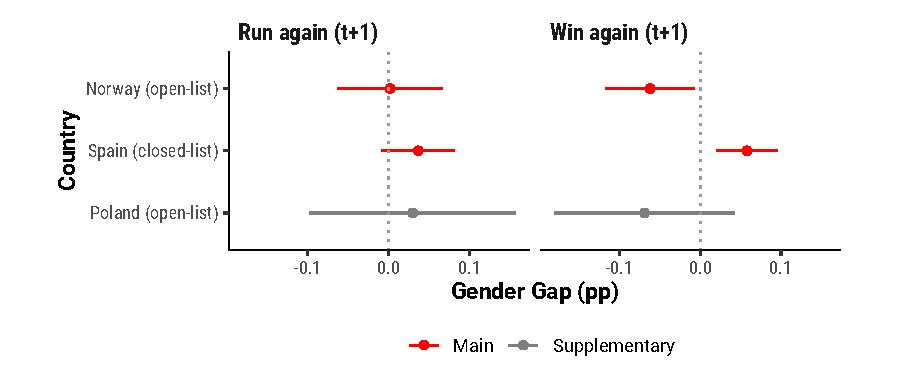
\includegraphics[width = 0.8\textwidth]{../output/figures/coef_summary.pdf}
    \caption{\textbf{Estimated Gender Gap in Incumbency Advantages Across Cases.} Point estimates from preferred difference-in-discontinuity specifications, with 95\% Confidence Intervals.}
    \label{fig:coef_summary}
\end{figure}


Figure \ref{fig:coef_summary} plots the difference in estimated incumbency effects between men and women for local elections in Norway (open-list) and Spain (closed-list), along with noisier, supplementary, estimates from Polish county-level elections (open-list).
There is no statistically significant gender gap in the effect of winning on running again in any country.
There is, however, a pronounced contrast in the effect on winning again: in Norway, women suffer from a far smaller incumbency advantage than their male colleagues (by about 7 pp), whereas female candidates in Spain experience a differentially larger incumbency advantage than men (by about 6 pp). Both estimates are statistically significant at conventional levels.
The gender gap under open-list PR likely replicates to similar settings outside Norway, as the results for Poland suggest (see Appendix \ref{app:poland}).

\begin{figure}[!htb]
    \centering
    \begin{subfigure}[t]{0.98\textwidth}
        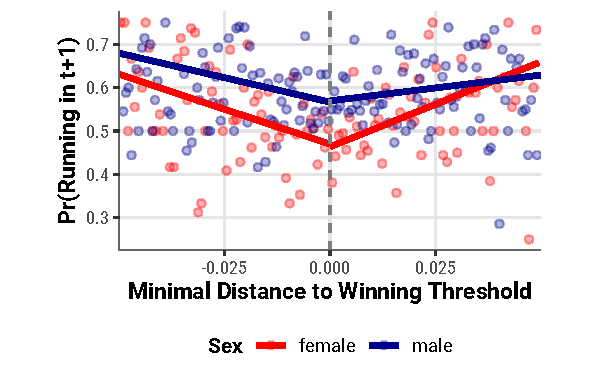
\includegraphics[width = 0.48\textwidth]{../output/figures/norway_run_again.pdf}
        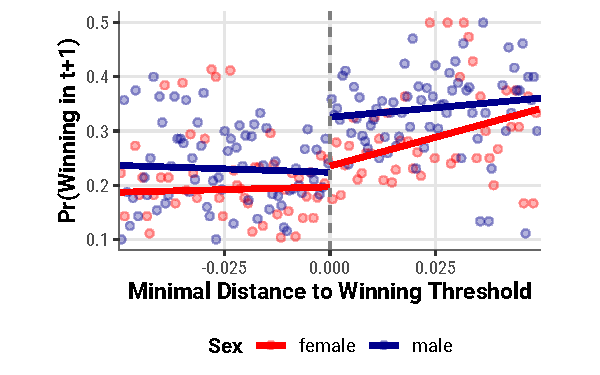
\includegraphics[width = 0.48\textwidth]{../output/figures/norway_win_again.pdf}
        \caption{Norwegian Local Elections \label{fig:main_plot_norway}}
    \end{subfigure}
    \begin{subfigure}[t]{0.98\textwidth}
        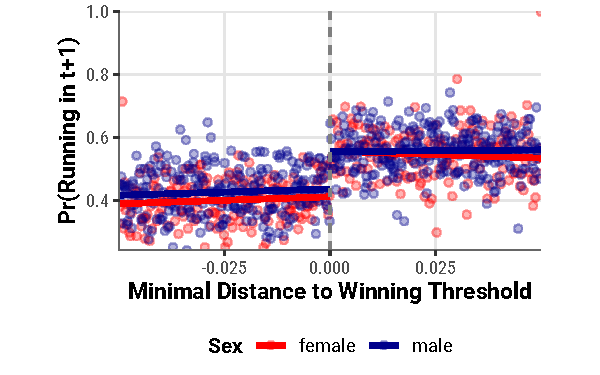
\includegraphics[width = 0.48\textwidth]{../output/figures/spain_run_again.pdf}
        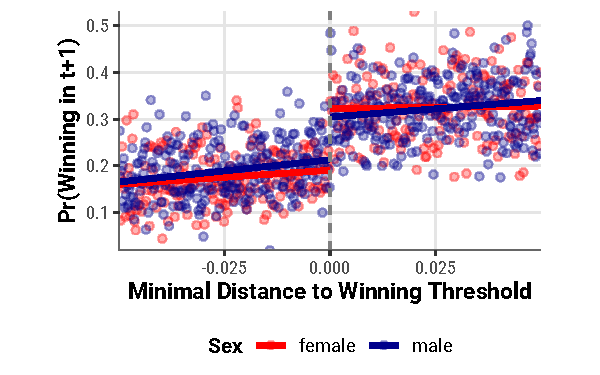
\includegraphics[width = 0.48\textwidth]{../output/figures/spain_win_again.pdf}
        \caption{Spanish Local Elections \label{fig:main_plot_spain}}
    \end{subfigure}
    \caption{\textbf{Effect of Winning Election on Running Again and Winning Again, By Gender And Case.} The visual regression discontinuities compare bare winners and bare losers by candidates' gender.}
    \label{fig:main_plot}
\end{figure}


Figure \ref{fig:main_plot} presents these findings in a graphical representation of the difference in discontinuities. Panel (a) shows the data from Norwegian open-list elections. Women, while unconditionally less likely to run again (left panel), do not suffer from any additional disadvantage in \emph{running again} compared to men once elected:
losing an election does not diminish women's persistence differentially. While barely winning increases the probability of \emph{winning again} for candidates of either gender (right panel), the effect is clearly greater for male candidates (4 percentage points for women vs. 10 percentage points for men). This matches the results from Figure \ref{fig:coef_summary}. Turning to Spanish closed-list elections in (b), we similarly observe no gender difference in the effect of winning on running again; candidates of either gender experience an increase of approximately 9 percentage points in the probability of winning again as a result of getting elected. Unlike in the Norwegian case, the Figure does not show a visually obvious gender gap; if anything, the effect appears somewhat larger for women.

In the remainder of this section, I parse these headline results in greater detail and provide additional results to guard against likely alternative explanations.

\subsection{Norway (Open-List PR)}

Turning to Norway's open-list elections first, Table \ref{tab:norway_main} backs up the graphical intuition with formal evidence in the form of difference-in-discontinuity estimates. Columns 1 to 3 report estimates of the effect of winning on running again in $t + 1$. Both the effect of being elected, as well as the gender gap coefficient, are close to zero across all bandwidth choices.

\begin{table}

\caption{\label{tab:norway_main} \textbf{Difference-in-Discontinuity Estimates For Incumbency Advantage In Norwegian Municipalities.} Women face diminished incumbency effect on winning again.}
\centering
\fontsize{9}{11}\selectfont
\begin{threeparttable}
\begin{tabular}[t]{lS[
              input-symbols=(),
              table-format=-1.3,
              table-space-text-pre    = (,
              table-space-text-post   = ),
              input-open-uncertainty  =,
              input-close-uncertainty = ,
              table-align-text-post = false]S[
              input-symbols=(),
              table-format=-1.3,
              table-space-text-pre    = (,
              table-space-text-post   = ),
              input-open-uncertainty  =,
              input-close-uncertainty = ,
              table-align-text-post = false]S[
              input-symbols=(),
              table-format=-1.3,
              table-space-text-pre    = (,
              table-space-text-post   = ),
              input-open-uncertainty  =,
              input-close-uncertainty = ,
              table-align-text-post = false]S[
              input-symbols=(),
              table-format=-1.3,
              table-space-text-pre    = (,
              table-space-text-post   = ),
              input-open-uncertainty  =,
              input-close-uncertainty = ,
              table-align-text-post = false]S[
              input-symbols=(),
              table-format=-1.3,
              table-space-text-pre    = (,
              table-space-text-post   = ),
              input-open-uncertainty  =,
              input-close-uncertainty = ,
              table-align-text-post = false]S[
              input-symbols=(),
              table-format=-1.3,
              table-space-text-pre    = (,
              table-space-text-post   = ),
              input-open-uncertainty  =,
              input-close-uncertainty = ,
              table-align-text-post = false]}
\toprule
\multicolumn{1}{c}{ } & \multicolumn{3}{c}{Run (t + 1)} & \multicolumn{3}{c}{Win (t + 1)} \\
\cmidrule(l{3pt}r{3pt}){2-4} \cmidrule(l{3pt}r{3pt}){5-7}
  & \multicolumn{1}{c}{(1)} & \multicolumn{1}{c}{(2)} & \multicolumn{1}{c}{(3)} & \multicolumn{1}{c}{(4)} & \multicolumn{1}{c}{(5)} & \multicolumn{1}{c}{(6)}\\
\midrule
Elected & 0.002 & -0.010 & 0.016 & 0.107 & 0.102 & 0.109\\
 & (0.019) & (0.016) & (0.024) & (0.017) & (0.015) & (0.021)\\
\addlinespace
Female & -0.097 & -0.092 & -0.085 & -0.027 & -0.024 & -0.026\\
 & (0.021) & (0.018) & (0.026) & (0.018) & (0.015) & (0.021)\\
\addlinespace
Elected x Female & 0.002 & 0.024 & -0.030 & -0.062 & -0.047 & -0.096\\
 & (0.033) & (0.028) & (0.039) & (0.028) & (0.024) & (0.034)\\
\addlinespace \midrule \addlinespace
Bandwidth & 0.054 & 0.11 & 0.027 & 0.05 & 0.099 & 0.025\\
BW Type & \multicolumn{1}{c}{Optimal} & \multicolumn{1}{c}{2x Opt} & \multicolumn{1}{c}{0.5x Opt} & \multicolumn{1}{c}{Optimal} & \multicolumn{1}{c}{2x Opt} & \multicolumn{1}{c}{0.5x Opt}\\
Outcome Mean & 0.564 & 0.575 & 0.551 & 0.261 & 0.263 & 0.257\\
N (left) & \multicolumn{1}{c}{4617} & \multicolumn{1}{c}{5529} & \multicolumn{1}{c}{3667} & \multicolumn{1}{c}{4502} & \multicolumn{1}{c}{5428} & \multicolumn{1}{c}{3549}\\
N (right) & \multicolumn{1}{c}{4666} & \multicolumn{1}{c}{5590} & \multicolumn{1}{c}{3711} & \multicolumn{1}{c}{4551} & \multicolumn{1}{c}{5489} & \multicolumn{1}{c}{3592}\\
\bottomrule
\end{tabular}
\begin{tablenotes}[para]
\item All estimates are reported with robust standard errors clustered at the municipality level in parentheses. Each observation is a candidate's election attempt. 'Elected' is an indicator for observations where the candidate obtained a seat in the municipal council. 'Female' is an indicator for observations identified as female. `Elected` times `Female` is the interaction between the two variables. Other coefficients (running variable) reported in Table I1. Regression run on all candidates in elections between 2003 and 2015. 
\end{tablenotes}
\end{threeparttable}
\end{table}

Columns 3 to 6 report the effect of winning on the probability of winning again in $t + 1$. For men, there is an increase of about 10 pp., which is statistically significant at all conventional levels. The interaction coefficient suggests that the incumbency advantage for women is approximately 6 pp. lower, which corresponds to a 60\% decrease in the magnitude of the effect. Although the precise magnitude of the difference between men and women varies between 5 and 10 pp. depending on the bandwidth, all interaction estimates are statistically significant.\footnote{For further robustness checks, Appendix \ref{app:bandwidth_sensitivity} reports the coefficients for a wide range of bandwidths. The results are also robust to dropping all municipalities in which some personal votes for candidates outside the threshold sample are recorded as missing (Appendix \ref{app:norway_restricted}), as well as to dropping outlying cities with very high populations (Appendix \ref{app:norway_outliers}).}

Together, these results constitute first evidence that female candidates in an open-list setting may suffer from a diminished incumbency advantage.

\subsection{Spain (Closed-List PR)}

I now turn to the results from closed-list elections in Spanish municipalities.

The formal estimates in Table \ref{tab:spain_main} corroborate the visual inspection and offer more precise results.
Once again, columns 1 to 3 report the effect of winning on running again in the next election.
There is a large and significant effect of winning on running again for men -- an approximately 10 percentage point increase, in line with the result from Figure \ref{fig:main_plot_spain}.
In this case, the gender gap is close to zero and statistically insignificant:
the effect of winning an election on running again appears to be of a very similar (or slightly larger in the case of some bandwidths) magnitude for women.

\begin{table}

\caption{\label{tab:spain_main} \textbf{Difference-in-Discontinuity Estimates For Incumbency Advantage In Spanish Municipalities}. Women likely enjoy a larger effect of winning on their probability to win again.}
\centering
\fontsize{9}{11}\selectfont
\begin{threeparttable}
\begin{tabular}[t]{lS[
              input-symbols=(),
              table-format=-1.3,
              table-space-text-pre    = (,
              table-space-text-post   = ),
              input-open-uncertainty  =,
              input-close-uncertainty = ,
              table-align-text-post = false]S[
              input-symbols=(),
              table-format=-1.3,
              table-space-text-pre    = (,
              table-space-text-post   = ),
              input-open-uncertainty  =,
              input-close-uncertainty = ,
              table-align-text-post = false]S[
              input-symbols=(),
              table-format=-1.3,
              table-space-text-pre    = (,
              table-space-text-post   = ),
              input-open-uncertainty  =,
              input-close-uncertainty = ,
              table-align-text-post = false]S[
              input-symbols=(),
              table-format=-1.3,
              table-space-text-pre    = (,
              table-space-text-post   = ),
              input-open-uncertainty  =,
              input-close-uncertainty = ,
              table-align-text-post = false]S[
              input-symbols=(),
              table-format=-1.3,
              table-space-text-pre    = (,
              table-space-text-post   = ),
              input-open-uncertainty  =,
              input-close-uncertainty = ,
              table-align-text-post = false]S[
              input-symbols=(),
              table-format=-1.3,
              table-space-text-pre    = (,
              table-space-text-post   = ),
              input-open-uncertainty  =,
              input-close-uncertainty = ,
              table-align-text-post = false]}
\toprule
\multicolumn{1}{c}{ } & \multicolumn{3}{c}{Run (t + 1)} & \multicolumn{3}{c}{Win (t + 1)} \\
\cmidrule(l{3pt}r{3pt}){2-4} \cmidrule(l{3pt}r{3pt}){5-7}
  & \multicolumn{1}{c}{(1)} & \multicolumn{1}{c}{(2)} & \multicolumn{1}{c}{(3)} & \multicolumn{1}{c}{(4)} & \multicolumn{1}{c}{(5)} & \multicolumn{1}{c}{(6)}\\
\midrule
Elected & 0.109 & 0.119 & 0.100 & 0.072 & 0.095 & 0.076\\
 & (0.014) & (0.010) & (0.020) & (0.012) & (0.008) & (0.017)\\
\addlinespace
Female & -0.024 & -0.032 & -0.012 & -0.032 & -0.026 & -0.033\\
 & (0.016) & (0.012) & (0.022) & (0.013) & (0.009) & (0.018)\\
\addlinespace
Elected x Female & 0.037 & 0.033 & 0.018 & 0.058 & 0.045 & 0.057\\
 & (0.023) & (0.017) & (0.032) & (0.019) & (0.013) & (0.027)\\
\addlinespace \midrule \addlinespace
Bandwidth & 0.032 & 0.064 & 0.016 & 0.035 & 0.071 & 0.018\\
BW Type & \multicolumn{1}{c}{Optimal} & \multicolumn{1}{c}{2x Opt} & \multicolumn{1}{c}{0.5x Opt} & \multicolumn{1}{c}{Optimal} & \multicolumn{1}{c}{2x Opt} & \multicolumn{1}{c}{0.5x Opt}\\
Outcome Mean & 0.486 & 0.483 & 0.485 & 0.256 & 0.251 & 0.254\\
N (left) & \multicolumn{1}{c}{14840} & \multicolumn{1}{c}{26294} & \multicolumn{1}{c}{7984} & \multicolumn{1}{c}{16223} & \multicolumn{1}{c}{28426} & \multicolumn{1}{c}{8726}\\
N (right) & \multicolumn{1}{c}{14729} & \multicolumn{1}{c}{26886} & \multicolumn{1}{c}{7825} & \multicolumn{1}{c}{16159} & \multicolumn{1}{c}{29072} & \multicolumn{1}{c}{8530}\\
\bottomrule
\end{tabular}
\begin{tablenotes}[para]
\item All estimates are reported with robust standard errors clustered at the municipality level in parentheses. Other coefficients (running variable) reported in Table I2. See Table 2 for additional details.
\end{tablenotes}
\end{threeparttable}
\end{table}

Columns 4 to 6 provide clear evidence that the incumbency effect on winning again is at least as great, if not bigger, for women.
Men experience an incumbency effect of an approximately 7 percentage point increase in their probability of winning the next election.\footnote{See Appendix \ref{app:rd_polynomial} for robustness to polynomial order, and Appendix \ref{app:bandwidth_sensitivity} for robustness to bandwidth choice. I also leverage the large number of observations in order to estimate a diff-in-diff sufficiently close to the threshold (within 1 percentage point) in Appendix \ref{app:spain_did}. The estimates are consistent with the results from Table~\ref{tab:spain_main}, and further point towards no large gender gap in the effect of winning on running again.} The gender gap coefficient is positive, and statistically significant at the optimal bandwidth (though not at other values), suggesting that the incumbency advantage is an additional 5 to 6 percentage points larger for women. This set of results suggests that women in Spanish local elections enjoy a somewhat \emph{greater} incumbency advantage than their male colleagues -- much in contrast to the findings in Norway's open-list PR setting.\footnote{In Appendix \ref{app:spain_by_party}, I check for any meaningful differences if I estimate the difference-in-discontinuity separately for either of Spain's two major parties. Second, in Appendix \ref{app:spain_by_quota}, I evaluate whether the results are meaningfully different for municipalities above that implemented a legally binding gender quota -- mandating that at least 40\% of all candidates be women -- versus those that did not. I do not find evidence of a negative gender gap for women across either type of municipality. In Appendix \ref{app:hetero_spain}, I also find no meaningful evidence that estimates differ by cities' population size, although the positive gender gap may be attenuated towards zero in cities in the highest population tercile.}

All told, the direct comparison between the results from Norway's open-list and Spain's closed-list elections is consistent with the theoretical argument that women suffer from disadvantages in incumbency effects where voters can determine individual candidates' list rankings. Still, on its own, this comparison cannot rule out that fundamental differences between Norway and Spain drive the set of results.

\subsection{Countries' Idiosyncracies Unlikely To Drive Gender Gap Difference}

Is the contrast in gender gap estimates the result of countries' idiosyncratic characteristics, rather than the product of electoral rules?

In Appendix \ref{app:case_extension}, I compare the gender gap in incumbency advantages across different electoral systems within the same country (Norway), and use the case of Poland's open-list local elections to demonstrate that the negative gender gap is not just an artefact of Norway's local politics.

Overall, the finding of a gender gap in incumbency advantages replicates for the same electoral system across different countries, but not for different electoral systems within the same country. This weakens (but cannot fully rule out) concerns about case selection driving the results and is consistent with the claim that differences in the type of proportional representation may affect the gender gap in political careers.

\subsection{Differential Selection Of Candidates Into Sample Unlikely To Drive Gender Gap}
\label{sec:diffsec}

In addition to concerns about the cross-country comparison discussed just above, we may also worry about threats to inference within any one case: if candidates' gender is also correlated with other characteristics, Norway's open-list results may simply reflect parties' or voters' preferences for the associated attribute, rather than gender itself \citep{bansak2021,teele2018}. Alternatively, female candidates in the threshold sample may run in different electoral environments (e.g. parties or geographies) that lead to smaller incumbency advantages \citep{folke2016a}. In both of these cases, differential selection into the sample could threaten the inference drawn from the observed gender gap.

I present two checks to guard against this explanation. First, I substitute gender with age and experience as conditioning variables in the difference-in-discontinuities setup in the Norwegian case.\footnote{Unfortunately, this is not possible to replicate in the Spanish case due to a lack of available candidate covariates.} My results in Appendix \ref{app:age_rd} suggest that there is no difference in the magnitude of the incumbency advantage between older and younger, or more and less experienced candidates.

Second, using a matching approach discussed in \citet{bansak2021} and \citet{bansak2022}, I compare female candidates to male candidates who are most similar on a number of individual- and election-level attributes. In Appendix \ref{app:matching}, I present results from various matched comparisons that remain consistent with my main findings.

Jointly, these results offer suggestive evidence that gender itself, rather than a correlated attribute, is a major factor driving the observed gender gap in incumbency advantages -- even though caveats about the finite nature of available covariates remain.

% -----------------------
% SECTION 5 - MECHANISMS
% -----------------------

\section{Mechanisms Behind the Gender Gap in Open-List PR}

What mechanism accounts for the stark difference in gender-specific incumbency advantages under open-list PR in Norway? In this section, I show that the gender gap is most pronounced among candidates in right-wing parties. I also find that voters in right-wing parties award a smaller increase in preference votes to female candidates as a result of being barely elected. This channel, mechanically unavailable in closed-list PR, is likely to contribute to women's smaller incumbency advantage in open-list settings. Put differently, this section provides suggestive evidence that the more candidate-centric nature of open-list PR opens the door to voter or systemic biases disproportionately affecting female candidates.

\subsection{Women's Disadvantage Concentrated in Right-Wing Parties}

\begin{table}[!h]

\caption{\label{tab:norway_by_party_inc} \textbf{Difference-in-Discontinuity Estimates For Incumbency Advantage In Norwegian Municipalities, By Political Party Group.}}
\centering
\fontsize{9}{11}\selectfont
\begin{threeparttable}
\begin{tabular}[t]{lS[
              input-symbols=(),
              table-format=-2.3,
              table-space-text-pre    = (,
              table-space-text-post   = ),
              input-open-uncertainty  =,
              input-close-uncertainty = ,
              table-align-text-post = false]S[
              input-symbols=(),
              table-format=-2.3,
              table-space-text-pre    = (,
              table-space-text-post   = ),
              input-open-uncertainty  =,
              input-close-uncertainty = ,
              table-align-text-post = false]S[
              input-symbols=(),
              table-format=-2.3,
              table-space-text-pre    = (,
              table-space-text-post   = ),
              input-open-uncertainty  =,
              input-close-uncertainty = ,
              table-align-text-post = false]S[
              input-symbols=(),
              table-format=-2.3,
              table-space-text-pre    = (,
              table-space-text-post   = ),
              input-open-uncertainty  =,
              input-close-uncertainty = ,
              table-align-text-post = false]}
\toprule
\multicolumn{1}{c}{ } & \multicolumn{2}{c}{Run (t+1)} & \multicolumn{2}{c}{Win (t+1)} \\
\cmidrule(l{3pt}r{3pt}){2-3} \cmidrule(l{3pt}r{3pt}){4-5}
  & \multicolumn{1}{c}{(1)} & \multicolumn{1}{c}{(2)} & \multicolumn{1}{c}{(3)} & \multicolumn{1}{c}{(4)}\\
\midrule
Elected & 0.022 & 0.005 & 0.086 & 0.126\\
 & (0.031) & (0.026) & (0.027) & (0.024)\\
\addlinespace
Female & -0.079 & -0.044 & -0.015 & -0.001\\
 & (0.034) & (0.030) & (0.027) & (0.025)\\
\addlinespace
Elected x Female & -0.040 & -0.014 & -0.053 & -0.089\\
 & (0.049) & (0.045) & (0.039) & (0.039)\\
\addlinespace \midrule \addlinespace
Parties & \multicolumn{1}{c}{Left} & \multicolumn{1}{c}{Right} & \multicolumn{1}{c}{Left} & \multicolumn{1}{c}{Right}\\
Bandwidth & 0.05 & 0.068 & 0.052 & 0.069\\
Outcome Mean & 0.546 & 0.59 & 0.253 & 0.26\\
N (left) & \multicolumn{1}{c}{1568} & \multicolumn{1}{c}{2382} & \multicolumn{1}{c}{1580} & \multicolumn{1}{c}{2388}\\
N (right) & \multicolumn{1}{c}{1589} & \multicolumn{1}{c}{2413} & \multicolumn{1}{c}{1601} & \multicolumn{1}{c}{2419}\\
\bottomrule
\end{tabular}
\begin{tablenotes}[para]
\item All estimates are reported with robust standard errors clustered at the municipality level in parentheses. Each observation is a candidate's election attempt. Other coefficients reported in Table I3.
\end{tablenotes}
\end{threeparttable}
\end{table}

Is the gender gap in the incumbency advantage persistent across parties from the entire spectrum of political ideologies? Both parties and voters following a more socially conservative ideology might be more inclined to exhibit a negative bias towards women, thus diminishing their incumbency advantage.\footnote{Appendix \ref{app:spain_by_party} repeats the same procedure for the Spanish case. } Although merely suggestive, a stark contrast between party families may also point towards voter bias, rather than universal, systemic bias, as a key mechanism.

I estimate the difference-in-discontinuity separately on subsamples of candidates from left-leaning and right-leaning parties and report the results in Table \ref{tab:norway_by_party_inc}.\footnote{Parties classified as 'left' are Labour and the Socialist Left. Parties classified as `right' are the Conservatives, (the right-wing populist) Progress, the Christian Democratic Party, and the Liberal Party, corresponding to the two 'coalition blocs' in Norwegian politics. I exclude the Centre Party, which has joined both left-wing and right-wing coalitions in recent decades.}  Columns 1 and 2 report the effect of winning on running again by subsample. Although noisier than the main results, we see the same finding replicated as in Table \ref{tab:norway_main}. There is no meaningful effect of being elected on running again in the next election for male candidates; nor is there a statistically significant difference in the effect between genders.

Columns 3 and 4 report the effect of winning on whether the candidate is elected in the next election. In left-wing parties, both the absolute incumbency effect for men, as well as the magnitude of the gender gap are smaller. Though the point estimate still suggests a 5 pp. lower incumbency advantage for women, the gender gap coefficient is no longer statistically significant in this subsample. By contrast, the gender gap is more pronounced in right-wing parties.

Here, male candidates who are bare winners enjoy an almost 13 percentage points higher chance of being re-elected (compared to male bare losers). For female candidates, however, this incumbency advantage is estimated to be almost 9 percentage points smaller, a statistically significant difference.


\subsection{Voters, Rather Than Party, May Drive Gender Gap}

Do party elites or voters drive the diminished incumbency advantage for women? Exploiting the specific rules of Norway's open-list elections, I fit the difference-in-discontinuity design on additional outcomes pertaining to the next election and provide suggestive evidence that right-wing voters' behavior contributes to the diminished incumbency advantage for women.

Recall that, party elites draw up an \emph{ex ante} ranking of candidates on the list, and award a \emph{pre-advantage} to select candidates (who receive a boost in preference vote shares as a result). However, if party elites are less likely to award these improvements to incumbent female candidates, this could explain the diminished incumbency advantage even though voters are no less likely to vote for women. Alternatively, if party elites exhibit no bias in the \emph{ex ante} placement of women, but there is a gender gap in the increase in preference votes awarded by voters upon winning the first time, then voters' male-favoring voting behavior may contribute to the diminished incumbency advantage for women.

\begin{table}[!h]

\caption{\label{tab:norway_by_party_mech} \textbf{Mechanisms leading to lower incumbency advantage: Difference-in-Discontinuity Estimates On Additional Outcomes, Norway.}}
\centering
\fontsize{9}{11}\selectfont
\begin{threeparttable}
\begin{tabular}[t]{lS[
              input-symbols=(),
              table-format=-2.3,
              table-space-text-pre    = (,
              table-space-text-post   = ),
              input-open-uncertainty  =,
              input-close-uncertainty = ,
              table-align-text-post = false]S[
              input-symbols=(),
              table-format=-2.3,
              table-space-text-pre    = (,
              table-space-text-post   = ),
              input-open-uncertainty  =,
              input-close-uncertainty = ,
              table-align-text-post = false]S[
              input-symbols=(),
              table-format=-2.3,
              table-space-text-pre    = (,
              table-space-text-post   = ),
              input-open-uncertainty  =,
              input-close-uncertainty = ,
              table-align-text-post = false]S[
              input-symbols=(),
              table-format=-2.3,
              table-space-text-pre    = (,
              table-space-text-post   = ),
              input-open-uncertainty  =,
              input-close-uncertainty = ,
              table-align-text-post = false]S[
              input-symbols=(),
              table-format=-2.3,
              table-space-text-pre    = (,
              table-space-text-post   = ),
              input-open-uncertainty  =,
              input-close-uncertainty = ,
              table-align-text-post = false]S[
              input-symbols=(),
              table-format=-2.3,
              table-space-text-pre    = (,
              table-space-text-post   = ),
              input-open-uncertainty  =,
              input-close-uncertainty = ,
              table-align-text-post = false]S[
              input-symbols=(),
              table-format=-2.3,
              table-space-text-pre    = (,
              table-space-text-post   = ),
              input-open-uncertainty  =,
              input-close-uncertainty = ,
              table-align-text-post = false]S[
              input-symbols=(),
              table-format=-2.3,
              table-space-text-pre    = (,
              table-space-text-post   = ),
              input-open-uncertainty  =,
              input-close-uncertainty = ,
              table-align-text-post = false]}
\toprule
\multicolumn{1}{c}{ } & \multicolumn{2}{c}{Orig. Rank Advance} & \multicolumn{2}{c}{Actual Rank Advance} & \multicolumn{2}{c}{Pre-Ad. (t+1)} & \multicolumn{2}{c}{Pers.V. Share (t+1)} \\
\cmidrule(l{3pt}r{3pt}){2-3} \cmidrule(l{3pt}r{3pt}){4-5} \cmidrule(l{3pt}r{3pt}){6-7} \cmidrule(l{3pt}r{3pt}){8-9}
  & \multicolumn{1}{c}{(1)} & \multicolumn{1}{c}{(2)} & \multicolumn{1}{c}{(3)} & \multicolumn{1}{c}{(4)} & \multicolumn{1}{c}{(5)} & \multicolumn{1}{c}{(6)} & \multicolumn{1}{c}{(7)} & \multicolumn{1}{c}{(8)}\\
\midrule
Elected & 0.088 & 0.066 & 0.026 & 0.044 & 0.037 & 0.058 & 0.003 & 0.005\\
 & (0.026) & (0.020) & (0.028) & (0.021) & (0.019) & (0.019) & (0.002) & (0.001)\\
\addlinespace
Female & 0.003 & -0.003 & -0.031 & 0.011 & 0.017 & 0.049 & -0.003 & 0.000\\
 & (0.027) & (0.023) & (0.029) & (0.023) & (0.022) & (0.021) & (0.003) & (0.002)\\
\addlinespace
Elected x Female & -0.063 & -0.034 & -0.013 & -0.062 & 0.001 & -0.041 & 0.001 & -0.005\\
 & (0.038) & (0.034) & (0.039) & (0.032) & (0.031) & (0.033) & (0.004) & (0.003)\\
\addlinespace \midrule \addlinespace
Parties & \multicolumn{1}{c}{Left} & \multicolumn{1}{c}{Right} & \multicolumn{1}{c}{Left} & \multicolumn{1}{c}{Right} & \multicolumn{1}{c}{Left} & \multicolumn{1}{c}{Right} & \multicolumn{1}{c}{Left} & \multicolumn{1}{c}{Right}\\
Bandwidth & 0.068 & 0.092 & 0.061 & 0.097 & 0.033 & 0.055 & 0.025 & 0.052\\
Outcome Mean & 0.257 & 0.253 & 0.229 & 0.211 & 0.119 & 0.163 & 0.0204 & 0.0175\\
N (left) & \multicolumn{1}{c}{1655} & \multicolumn{1}{c}{2620} & \multicolumn{1}{c}{1624} & \multicolumn{1}{c}{2662} & \multicolumn{1}{c}{1421} & \multicolumn{1}{c}{2203} & \multicolumn{1}{c}{446} & \multicolumn{1}{c}{840}\\
N (right) & \multicolumn{1}{c}{1676} & \multicolumn{1}{c}{2655} & \multicolumn{1}{c}{1645} & \multicolumn{1}{c}{2698} & \multicolumn{1}{c}{1441} & \multicolumn{1}{c}{2229} & \multicolumn{1}{c}{458} & \multicolumn{1}{c}{856}\\
\bottomrule
\end{tabular}
\begin{tablenotes}[para]
\item All estimates are reported with robust standard errors clustered at the municipality level in parentheses. Each observation is a candidate's election attempt. Other coefficients reported in Table I4.
\end{tablenotes}
\end{threeparttable}
\end{table}

Table \ref{tab:norway_by_party_mech} reports the results.
Because previous results suggest that the gender gap is most pronounced in right-wing parties, I fit the specification separately on left-wing and right-wing candidates.\footnote{The results are substantively similar when fitting second-order polynomials (Appendix \ref{app:norway_mech_poly}).}

In columns 1 and 2, I investigate whether winning an election renders candidates more likely to advance in \emph{ex ante} list rank in the next election. Across both left- and right-wing parties, male winners enjoy a significant increase in their probability of improving their ex ante rank as a result of winning. I find no statistically significant gender gap, although the point estimates are still signed negative.
In columns 3 and 4, examine whether candidates advanced in \emph{ex post} ranks -- after voters cast their preferences. In left-leaning parties, neither men nor women enjoy a statistically significant effect. By contrast, in right-wing parties, male winners are 4 percentage points more likely to improve their ex-post rank in the next election. The gender gap, close to significant at conventional levels, suggests that this effect is 6 percentage points \emph{lower} for women. Contrasting this with the previous columns, it suggests that most of the diminished incumbency advantage that women face in right-wing parties comes from voters.

Another way of examining whether party elites are responsible for holding back female winners is to look at awarding pre-advantage status. Columns 5 and 6 suggest that men enjoy an increased probability (4 to 6 pp.) of receiving pre-advantage status when elected. In neither case, however, do we find a statistically significant gender gap in the effect of being elected on attaining pre-advantage.

Finally, I turn to the effect of winning on the share of preference votes received in the next election.\footnote{\label{fn:pv_robust}These estimates report the effect on the share of preference votes \emph{relative to all votes cast in the municipality}. Measuring personal votes is somewhat more challenging than previously discussed binary outcomes.
Appendix \ref{app:norway_pv_estimation} shows robustness to different operationalisations of personal vote measures.} For these specifications, I drop municipalities flagged as having incomplete personal vote records and condition the sample on running again in the first place.\footnote{
    Unlike previous binary outcomes, it is less clear that imputing "0" personal votes for those not running again is justifiable. Following \citet{demagalhaes2015}, conditioning is only problematic if barely elected and barely defeated candidates exhibit different probabilities of running again, which I do not observe in this context. Appendix \ref{app:norway_pv_data} discusses the sample restriction further and shows that results are consistent (though noisier) when including all observations.
} On average, male left-wing candidates, upon being elected, can expect a 0.3 percentage point (0.5 in right-wing parties) higher preference vote share in the next election. While the estimate is small in absolute size, it is meaningful in relation to candidates' average preference vote share of 2 (1.75) percentage points, representing a 15\% (28\%) increase for the average candidate in the sample. We see a stark difference in the estimated gender gap between the two party groups. In left-wing parties, the coefficient is close to zero, whereas in right-wing parties, it is negative, statistically significant, and drives the incumbency advantage in preference votes for women back to zero.

Overall, these results, though with the caveat of large uncertainty, point towards right-wing voters rewarding female candidates for being elected with a smaller increase in personal votes as an important factor in explaining the gender gap. An increase in personal votes as a meaningful incumbency advantage mechanism may thus not be available to all candidates to the same extent \citep{fiva2018a}. Although I cannot precisely estimate whether women also face diminished effects for outcomes solely determined by party leadership, my results suggest that, at worst, both voters and party elites -- perhaps responding strategically -- play a role in decreasing women's incumbency advantage.

\section{Conclusion}

Do different forms of proportional representation feature gender gaps in political careers? This paper is among the first to evaluate gender gaps in incumbency advantages under PR.
Under closed-list PR, voters are unable to determine individual candidates' list positions: consequently, female candidates are likely shielded from voters' biases and experience incumbency effects that are equal to or greater than men's. Meanwhile, under open-list PR, female candidates may suffer from diminished incumbency advantages as incumbency effect mechanisms operate through voter-based name recognition channels, which may be more vulnerable to gender stereotyping. I provide direct evidence of the contrast in incumbency gender gaps between open- and closed-list PR; and also offer suggestive evidence that voters' ability to choose between individual candidates in open-list PR allows for voter or systemic biases to enter and hold back women's incumbency advantages.

Jointly, the results in this paper point towards the role that electoral rules play not only for the \emph{overall} share of women elected but also whether female candidates, once elected, enjoy equitable political careers. This finding highlights how gender imbalances can remain present through differential incumbency advantages and higher turnover even if the overall share of women elected begins to reach full equality. It may also help explain why, despite an increase in the nominal share of women, downstream outcomes such as municipal fiscal policy might not change \citep{ferreira2014,bagues2020}. Overall, this suggests that electoral systems which achieve nominally equitable descriptive representation may not guarantee fully equitable substantive representation.

The paper's findings come with caveats that also point towards promising avenues for future research. First, more work is needed to provide more direct and more precise evidence for theorized mechanisms.
Second, additional work is also needed to test whether my findings generalize beyond the selected cases, in particular with respect to other variants of open-list (and flexible-list) PR. This is especially important as other countries use different forms of this family of electoral systems: these variants vary in the degree to which they allow voters to rank individual candidates, and may therefore also affect the magnitude of the incumbency gender gap. Lastly, we should also research the gender gap in women's promotion to higher-ranked offices, thus studying whether the `leaky pipeline' is indeed responsible for women's underrepresentation in higher levels of politics, and compare the results with similar studies under plurality \citep{wasserman2020,brown2019,cipullo2021}.

It is also important to emphasize that, even beyond concerns about limiting voter's influence over who gets elected, closed-list PR is far from a panacea for equal representation: even with improved incumbency advantages, women are still a far way off from achieving equal representation. Further research is also needed into whether female candidates achieve similar rates of promotion into more senior offices, and whether parties still select female candidates strategically \citep{verge2019parties}. Put differently, my results do not speak to the problem of `sticky floors' \citep{cipullo2021}: women may struggle to get elected in the first place, and parties might still disadvantage women \emph{unconditionally} by placing them in lower or unwinnable ranks. Still, this paper demonstrates that parties, policymakers and electoral reformers should also consider the impacts of electoral systems on gender differences throughout candidates' entire career trajectory.


\singlespacing

\setstretch{0.6}
\setlength\bibsep{3pt}
\renewcommand*{\bibfont}{\small}
\bibliographystyle{apsr_fs.bst}
\bibliography{Spain_Careers.bib}

\end{document}
